\section{실험 과정}

\subsection{준비}
$\rm{CsPbBr_3}$ 용액은 실온 1기압 상태에서 제작되었다. $\rm{CsPbBr_3}$의 용액을 만들기 위해서 $\rm{CsBr}$과 $\rm{PbBr_2}$를 1:1의 몰 비율로 $\rm{CsBr}$ 0.638g과 $\rm{PbBr_2}$ 1.101 g을 섞었으며 용매인 Dimethyl Sulfoxide (DMSO) 6ml에 섞었다. 용매와 용질을 균일하게 섞기 위해서 50ml들이 통에 담은 후 뚜껑 부분을 파라필름으로 밀봉하고, 통을 물이 담긴 비커에 담은 후 초음파 분쇄기에 3분간 넣었다. 

\begin{figure}[h]
	\begin{center}
		\begin{tabular}{ccc}
			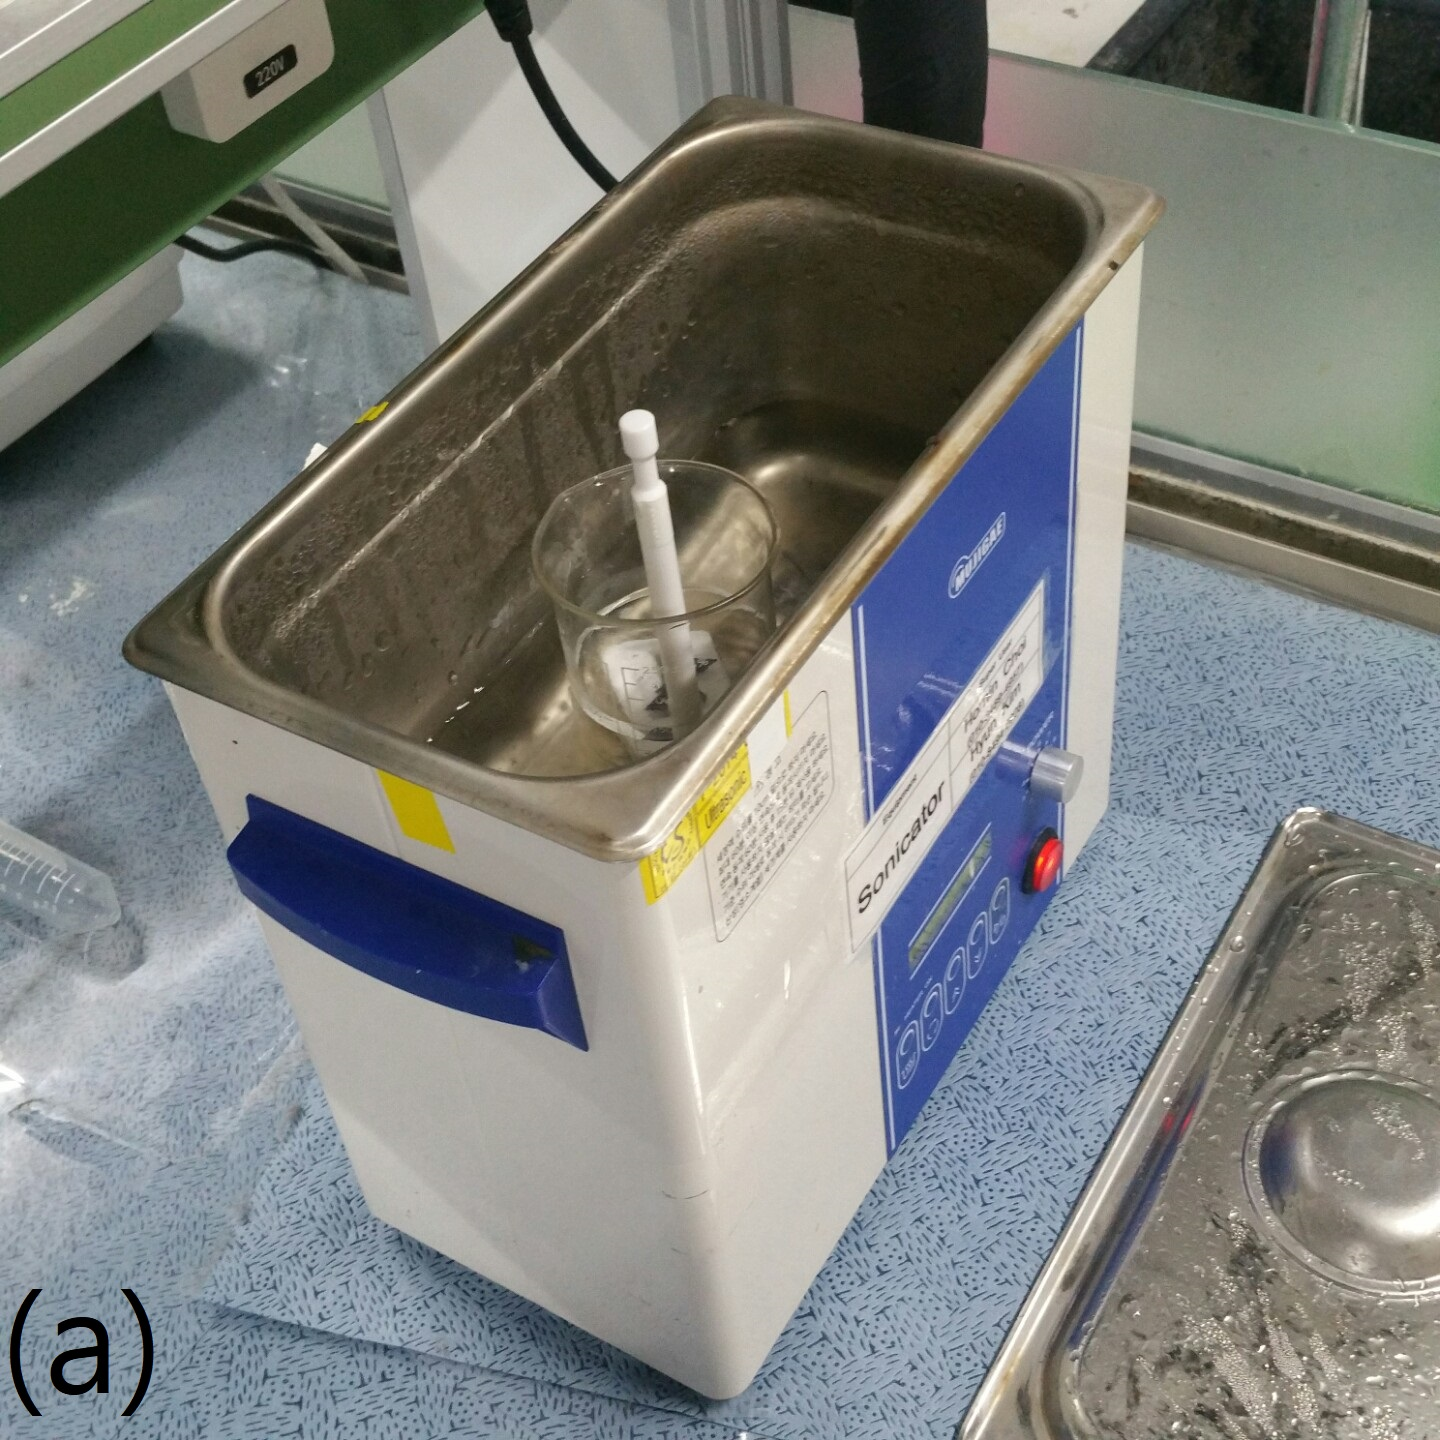
\includegraphics[width=4cm]{sonic} &   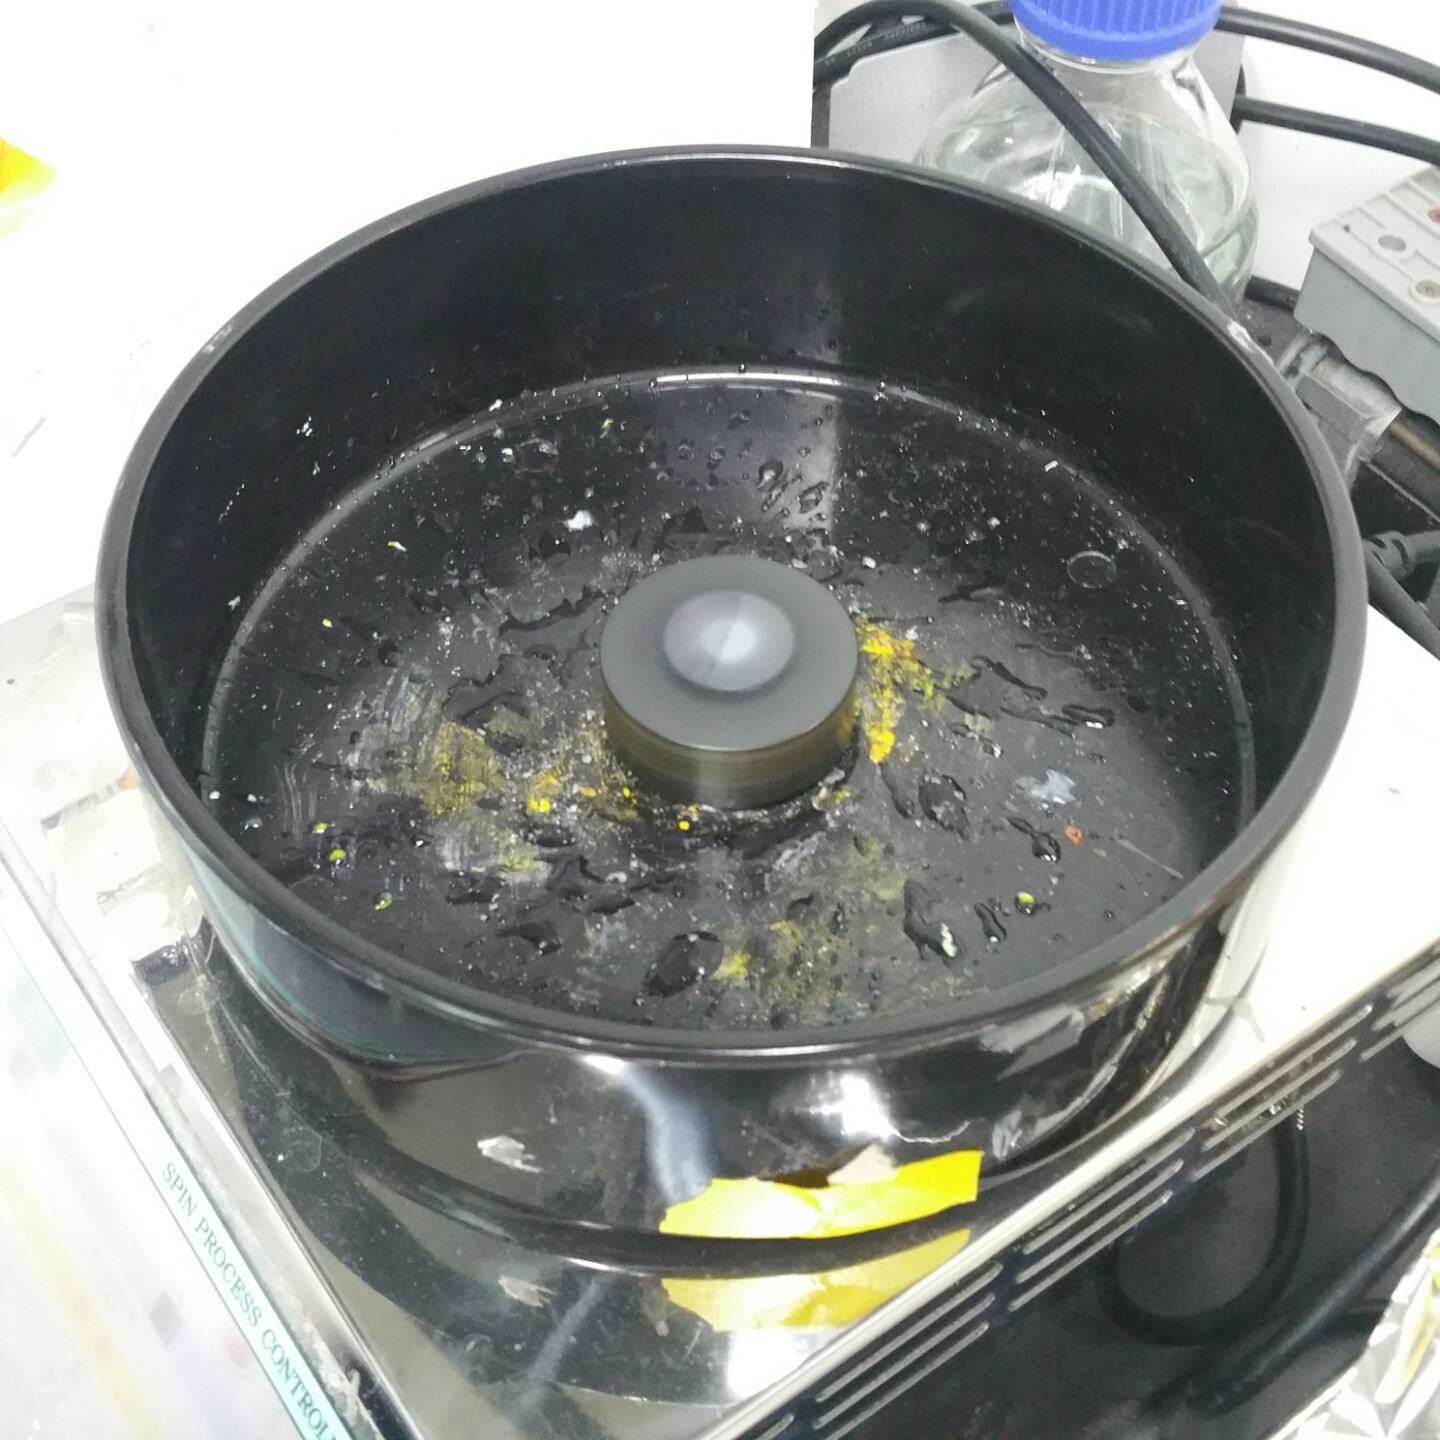
\includegraphics[width=4cm]{spin_coater} &
			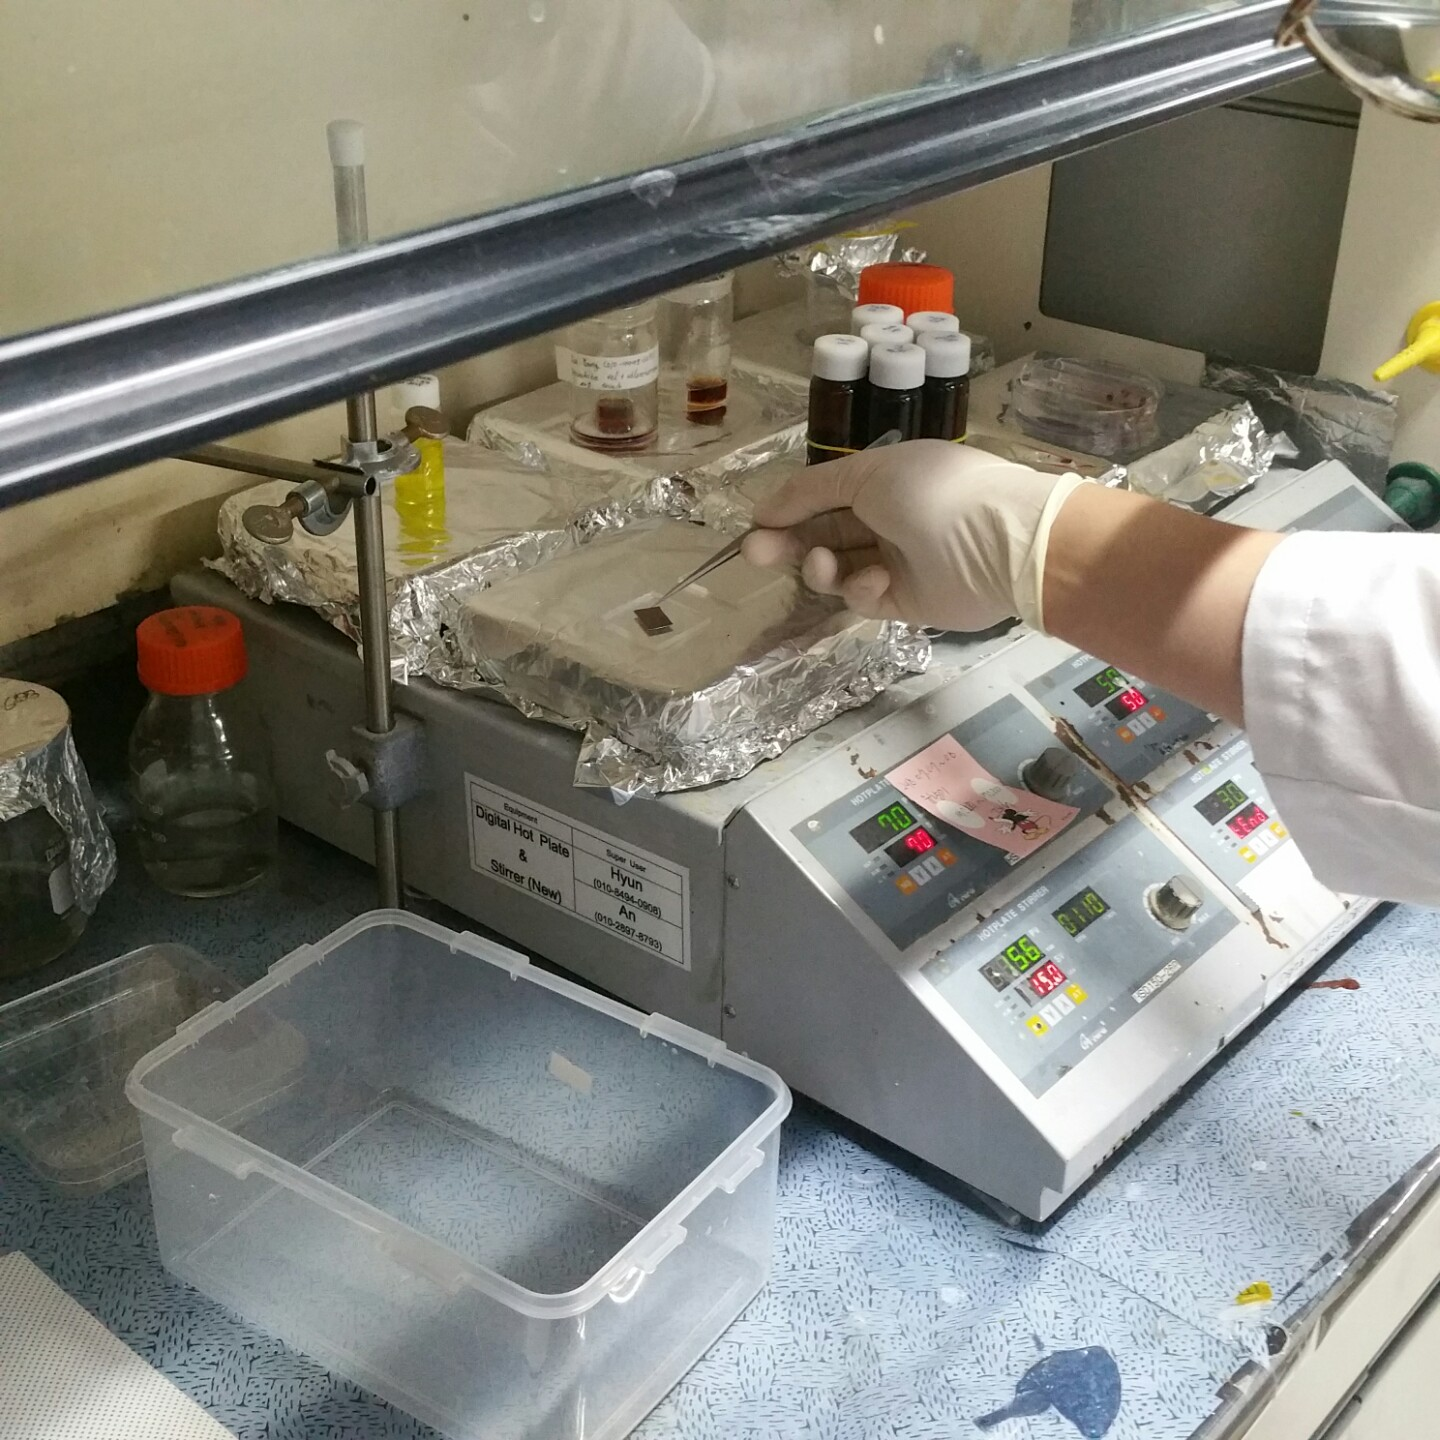
\includegraphics[width=4cm]{pdms_stamping}
		\end{tabular}
	\end{center}
			\begin{tikzpicture} [remember picture,overlay]
			\node[text=white] at (1.2, 4.3) {(a)};
			\node at (5.2, 4.3) {(b)};
			\node[text=white] at (10.0, 4.3) {(c)};
			\end{tikzpicture}	
		\caption{(a) Sonication process was held for 3 minutes. (b) Spin coater was used to outspread the solution equally on the silicon wafer. (c) PDMS was stamped onto the silicon wafer with $\rm{CsPbBr_3}$ solution. }	
		\label{fig:FIR102}
\end{figure}
또, 초음파 분쇄기를 이용하여 세척한 Silicon wafer 위에 $\rm{O_2}$ plasma를 이용하여 wafer 표면을 친수성으로 만들어 준 후 2000 rpm으로 1분간 spin coating을 이용하여 용액을 균일하게 펼쳐주었다. 마지막으로 미리 \SI{100}{\celsius}로 예열한 핫플레이트에서 5분간 PDMS를 이용하여 눌러주었다. PDMS위에 200g의 무게를 올려놓아 stamping이 잘 일어나도록 하였다. \\

\subsection{분석}
$\rm{CsPbBr_3}$ 결정이 만들어졌는지 광학현미경으로 확인한 후, X선 회절법과 TRPL 분석을 진행하였다. XRD measurement는 BRUKER사의 SmartLab 모델을 이용하였고, 입사각을 10°에서 70°까지 변화시키면서 측정하였다. 또, PL과 TRPL는 NT-MDT II Ntegra Spectra DUO Max라는 모델을 이용하여 가장 짧은 파장인 405nm 레이저로 측정을 하였다. 각각 ND0, ND1필터를 이용해서 측정하였으며, 그 이유는 .
